\documentclass[11pt]{article}
\usepackage{common}
\title{Musical Accompaniment}
\author{Amy Gu and Brian Yu}
\date{December 8, 2017}
\begin{document}
\maketitle{}


\section{Introduction}

Our system is a musical accompaniment program that accepts
an audio file of a soloist's musical performance as input,
and produces a new audio file that overlays the soloist's performance
with musical accompaniment. The system attempts to match the soloist's
performance in pace and volume to create harmonious accompaniment.

More specifically, the goal of our system is to take an
audio waveform input and intelligently identify the most likely
places in that audio where notes of a musical score appear,
given that the system already has an internal representation
of the musical score to begin with. We also hope to learn the
relative volumes at which the soloist plays different dynamics
in the piece, such that the system can emulate those dynamics
when playing the accompaniment.

The scope of our system is limited to soloist performances in which
only one note is played at any given point in time.
This avoids needing to disambiguate multiple notes when played
as a chord, and also simplifies the emission model and
transition model to allow for
states represented only by a single note.

The actual implementation of this system focuses on inference
using Hidden Markov Models for pitch inference and unsupervised
learning using k-means clustering for learning the musical
dynamics.

\section{Background and Related Work}

This inspiration for our implementation comes from Pardo and Birmingham
\cite{pardo}, who propose the representation of music as a Hidden
Markov Model and divide the problem of score following into two
components: transcription and alignment.
Pardo and Birmingham also suggest usage of the Viterbi algorithm,
though they adapt the algorithm for on-line use at a single point
in time, while we adapt our own algorithm for determining the
most likely sequence of musical states across the entire time
of the piece.

Dannenberg \cite{dannenberg} also proposes an algorithm for determining
the most likely sequence of musical states, but makes a (not unreasonable)
assumption that the actual performance events will not deviate much
from the score. In order to allow for noisy audio files and imperfect
playing that deviates from the score, we implement our own algorithm
without this assumption.

The use of k-means for dynamics detection is our own novel approach,
and is based on an attempt to identify clusters of dynamically
similar notes for purpose of emulation during accompaniment,
such that players who naturally play louder, softer, or naturally
have larger or smaller differences between their dynamics are
accommodated.

\section{Problem Specification}

The first stage of the problem is mapping the notes of the musical
score to specific time offsets in the source audio file.
To do this, we represent our musical piece as a Hidden Markov Model.
The hidden states are the actual note in the musical score at which
the soloist is playing at a given point in time. The emission states
are the observed performance information that we gather about what sound
we hear at a given point in time. Using this information, we need then
compute the most likely sequence of assignments of note numbers to
each of our observed states to determine when each note in the score
is actually being played.

The next stage of the problem is identifying the player's
musical dynamics. Here, our input is the velocity at which a particular
soloist played each note in a piece, as well as the number of different
dynamic categories (forte, mezzo forte, etc.) in the piece. The output
is an assignment of each dynamic category to an expected velocity
that best characterizes that dynamic category for the given soloist's
performance.

\section{Approach}

In order to initially convert our audio waveform to a quantifiable
representation of likely performance events, we use the open-source
aubio library to perform a Fast Fourier Transform on the waveform
to then extract likely performance events.

Those performance events then become the states of the Hidden Markov
Model, with each event demarcating a different time step in the piece.
We also add a performance event 0 to denote the performance event
of the start of the score before the first note.
Hidden state values (i.e. the actual notes in the score)
are numbered according to their ordering in the original piece,
with an additional hidden state 0 added to represent the state for
time steps before the beginning of the first note. Emission states are
the observed pitches.

Then, we run Viterbi's Algorithm to compute the
most likely sequence of states in the Hidden Markov Model given all
of our evidence for the entire piece.
Once we have a computation of the most likely sequence of states,
we can directly translate the state changes wherein the score note
also changes as the time at which one note changes into another.

We chose an initial emissions and transition model based on
intuitively reasoning about the nature of the model. Our emissions
model behaves as follows: we start by weighting all emissions equally
weighted with weight 1.
Then, we add 10 to the weight of the emission probabilities of emissions
that are two semitones away from the hidden note, 20 to the weights
for emissions that are one semitone away from the hidden note, and 30
to the weight of the emission corresponding to the hidden note exactly.
This distribution is then normalized, and the resulting distribution
is the emission model.

Our transition model follows this behavior: if starting at state $i$, the weight
of the transition distribution of moving to state $i+j$ is $j$ for all $j > 1$ up through
the end of the number of states. Call the sum of the weights as of this point $s$.
Then, the weight of state $i + 1$ is $2s$ and the weight of state $i$ is $s$.
Intuitively, this means we have about a 0.5 chance of moving to the next note, a 0.25
chance of staying at the same note, and a 0.25 chance of skipping some number of notes,
weighted more havily towards skipping fewer notes.

For computation of dynamics, we use the following algorithm, which relies
upon k-means:

\begin{algorithm}
  \begin{algorithmic}
    \Procedure{Dynamics}{$configuration$, $observations$}
    \State{$k \gets $ number of distinct dynamics in $configuration$}
    \State{$dynamics \gets $ \{ note.velocity : note $\in$ observations \} }
    \State{$clusters \gets$ K-MEANS($dynamics$, $k$) }
    \State{$results \gets$ \{ cluster.median : cluster $\in$ clusters \} }
    \State{return $results$}
    \EndProcedure{}
  \end{algorithmic}
  \caption{Dynamics calculation algorithm.}
\end{algorithm}

In effect, this algorithm uses k-means to cluster the note velocities into
as many clusters as there are distinct dynamic notations in the musical score,
and then takes the median of those clusters as the dynamic to use when
playing accompaniment.

In order to generate the accompaniment, we generate a MIDI file with
pre-determined accompaniment notes played at times given by the timesteps
corresponding to note changes in the most likely sequence of states generated
by Viterbi's Algorithm. Then, we convert the MIDI file to a WAV file,
and then overlay the accompaniment WAV file with the original WAV file,
removing the temporary files after completion.

\section{Experiments}

In order to analyze the effectiveness of our algorithm, we recorded 60
samples of the first 30 notes of Ode to Joy played on the piano by a human
performer. For the first 30 audio samples
(hereafter referred to as the ``good'' samples), each note was played correctly,
though different samples varied in pace, volume, and dynamic changes in order
to test the algorithm's performance under conditions that were meant to approximate
the way different performers might perform the same piece of music.

For the second 30 audio samples (hereafter referred to as the ``bad'' samples),
mistakes were intentionally added to the performance in order to test the algorithm's
robustness against imperfect soloist performance: some notes were added,
others removed, others changed to a different note, for instance.

Since each sample of Ode to Joy contained 30 notes across 60 pieces,
in total our implementation
was tested on 1800 distinct soloist note articulations.

We ran each sample through our harmonizer to generate accompaniment audio,
and then listened to each one, counting the number of errors, where an error is
defined as a note played by the accompaniment that did not align with the correct
corresponding note in the soloist performance. For incorrect notes played by
the soloist, whatever the accompaniment attempted to play during that time step
was not marked incorrect, unless such a mistake caused some future mistake to be
played alongside a correct note.

Our algorithm is also capable of handling songs other than Ode to Joy by specifying
an appropriate configuration file that describes what notes to expect and what
accompaniment to play alongside it. Much of our initial testing was done using
the first few notes from You'll Be Back from the musical Hamilton, for instance.

\subsection{Results}

Out of the 900 notes played in the good samples, 833 were accompanied correctly,
for an overall accuracy of about 92.6 percent. Out of the 900 notes played in the
bad samples, 827 were accompanied correctly, for an overall accuracy of about 91.9
percent.

In all cases, for a 30 note piece, each sample was accompanied by an accompaniment
track that had between 0 and 5 musical errors (inclusive), with most accompaniment
tracks having between 1 and 3 musical errors.

A graph of the distribution of the number of errors across each of the audio samples,
divided by good and bad samples, is shown below:

 \centerline{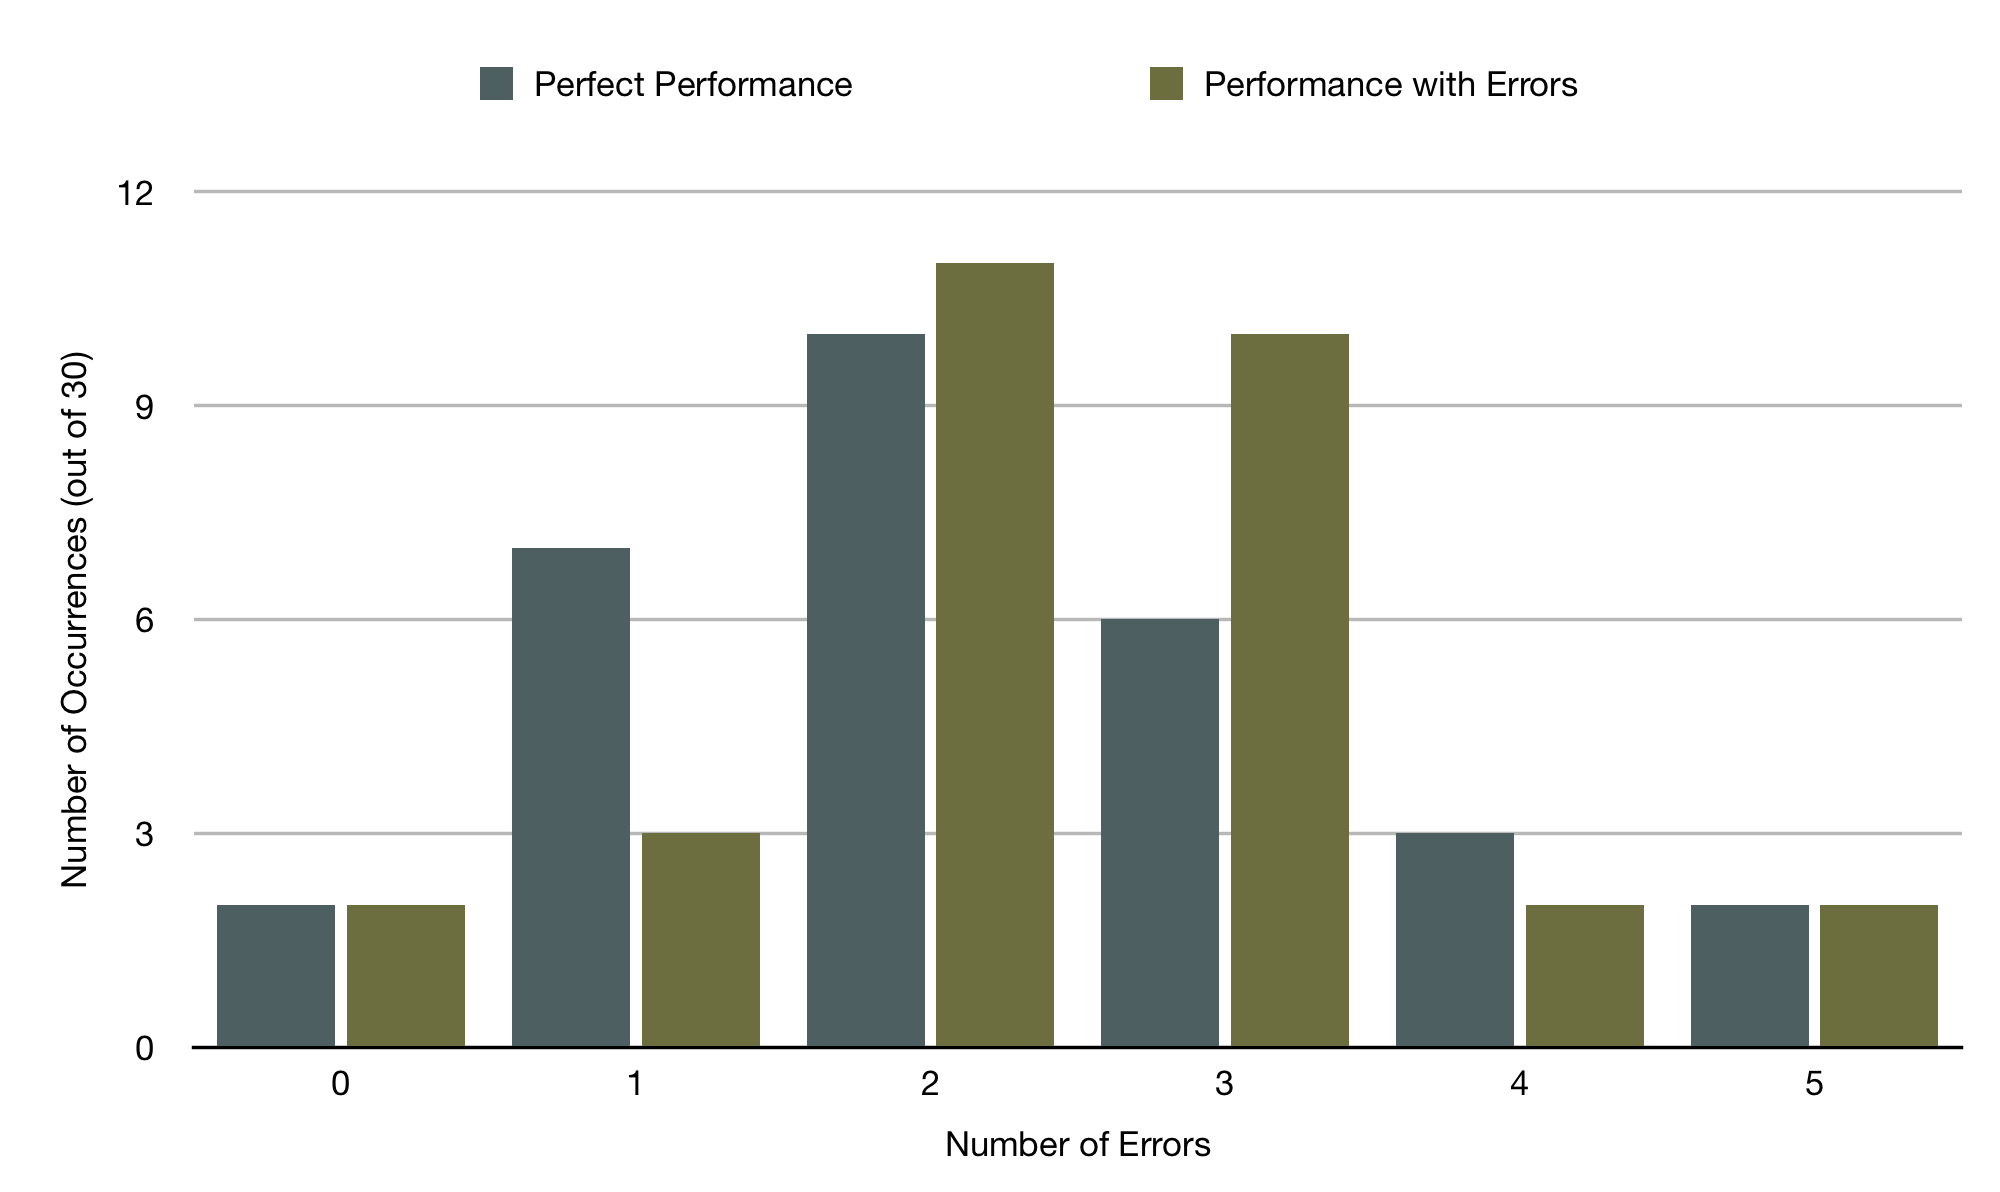
\includegraphics[scale=0.4]{graph.png}}

\section{Discussion}

On the whole, our system is fairly consistently (85 percent of the time)
able to accompany a 30-note
performance with three or fewer errors, for an accuracy rate within the piece
of 90 percent or higher.

Interestingly, our system's accuracy doesn't change much even for inaccurate
soloist performances. For our good samples, the average number of errors
in the accompaniment was 2.23 for each sample. In comparison, for the bad samples,
average number of errors in the accompaniment was 2.43 per sample, demonstrating
a slight loss in accuracy but only by 0.2 errors per sample on average.

Throughout the various accompaniment pieces, there were common patterns as to where
errors were most likely to take place.
More than 75 percent of the errors took place when the original piece had two of the
same note played immediately after each other.
In particular, many of these recorded errors during our testing involved failing to
match the second of the two matching notes with an accompaniment note, or trying to match
two accompaniment notes with the first of the matching notes. This is likely due to
the fact that, since our sensor model will often detect two articulated versions of
the same note even when only a single note is played, it's difficult for our algorithm
to tell apart when a note has actually been played twice versus just sensed twice
by our sensor model. This issue is compounded for certain instruments, like the violin,
where articulation of the same note played multiple times can be less clear.

Despite the issue that the algorithm had with detecting two notes immediately
in sequence, it was quite good at correcting itself: in almost all cases, immediately
after an error involving a sequence of two identical notes, the accompaniment
returned to playing the correct sequence of accompaniment notes (except in cases
where another error was observed).

Because our Hidden Markov Model only bases its transition probabilities
on the current state (i.e. the pitch that is currently being played), it doesn't
take into account additional information which may be helpful for determining
whether the soloist is likely to move on to the next note; in particular,
the model doesn't currently factor in how long a particular note has been playing for
into the computation for what the likelihood of moving to the next note is.
Intuitively, it's reasonable to argue that if a note has been playing for a longer
amount of time, there's a higher likelihood that the player will move on to the next note,
especially if a given score tells us how long we expect each note to last in terms
of a number of beats. Using a variant on the Hidden Markov Model that bases transition
probabilities on the prior $n$ states rather than just the prior 1 might be helpful
in this respect to improve the accuracy of the accompaniment.

\appendix

\section{System Description}

This system requires Python 3, with the following Python libraries (which are pip installable, and also found in requirements.txt): \texttt{aubio}, \texttt{midi2audio}, \texttt{MIDIUtil}, \texttt{pydub}. The generation of the audio also requires the installation of ffmpeg and fluidsynth, which are brew installable on Mac computers via the commands \texttt{brew install ffmpeg} and \texttt{brew install fluidsynth --with-libdsnfile}. In the latter case, the command line argument is necessary in order to install a sound font that is used to convert MIDI files to WAV files: if installing fluidsynth manually without brew, it's necessary to also install a soundfont (available on fluidsynth's website).

Once all dependencies are installed, you'll need to set up a \texttt{.json} file
for the song configuration you wish to process audio for. Two samples are already provided in
\texttt{ode.json} and \texttt{hamilton.json}. To run the program on an audio file other
than those two pieces (not necessary if you want to just test the implementation
on the two provided configurations),
format each \texttt{.json} file as a JSON object with two keys:
\texttt{piece}, which is a list of dictionaries of \texttt{pitch}es and \texttt{vel}s
(velocities), and \texttt{accompaniment}, which is a dictionary mapping strings
representing indices into the piece with a list of the desired MIDI pitches to play
at that note.

Next, you'll need a \texttt{.wav} file recording of a soloist's performance of the piece.
Some samples are provided in the \texttt{wav} directory already for testing purposes,
but you may also record arbitrary wav files of our own.

To actually run the system, use the command
\texttt{python harmonize.py CONFIGFILE AUDIOFILE}, where
\texttt{CONFIGFILE} is the path to the configuration file for the piece
(e.g. \texttt{config/ode.json})
and \texttt{AUDIOFILE} is the path to the audio WAV file for the piece
(e.g. \texttt{wav/ode1.wav}).

The produced audio file will be saved as \texttt{output.wav}, which will
be an audio file that contains both the original audio as well as the system-generated
accompaniment soundtrack.

\section{Group Makeup}

Amy: focused mostly on learning the dynamics model for the accompaniment
system and devising the k-means variant used to perform those computations,
and worked on tuning the parameters of the Hidden Markov Model to improve
the accuracy of the system.

Brian: focused mostly on implementing Viterbi's Algorithm and devising
the initial models for the dynamics of the musical system, as well as
experimentation and testing.

\bibliographystyle{plain}
\bibliography{bibliography}

\end{document}